\documentclass{article}
\usepackage{amssymb}
\usepackage{graphicx}
\usepackage{svg}

\begin{document}
\title{\vspace{-60pt}Assignment 1: Design\vspace{-2ex}}
\author{Joshua Dong}
\date{\vspace{-2ex}\today}
\maketitle

\section{System IPO}
\vspace{-12pt}
\begin{figure}[h]
  \centering
  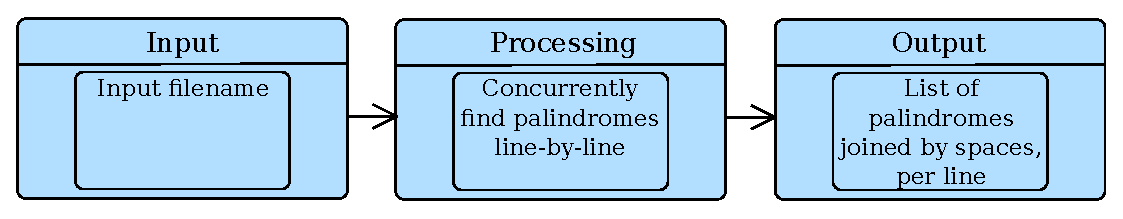
\includegraphics[width=0.9\textwidth]{IPO.eps}
\end{figure}


\section{Functional Block Diagram}
\vspace{-12pt}
\begin{figure}[h]
  \centering
  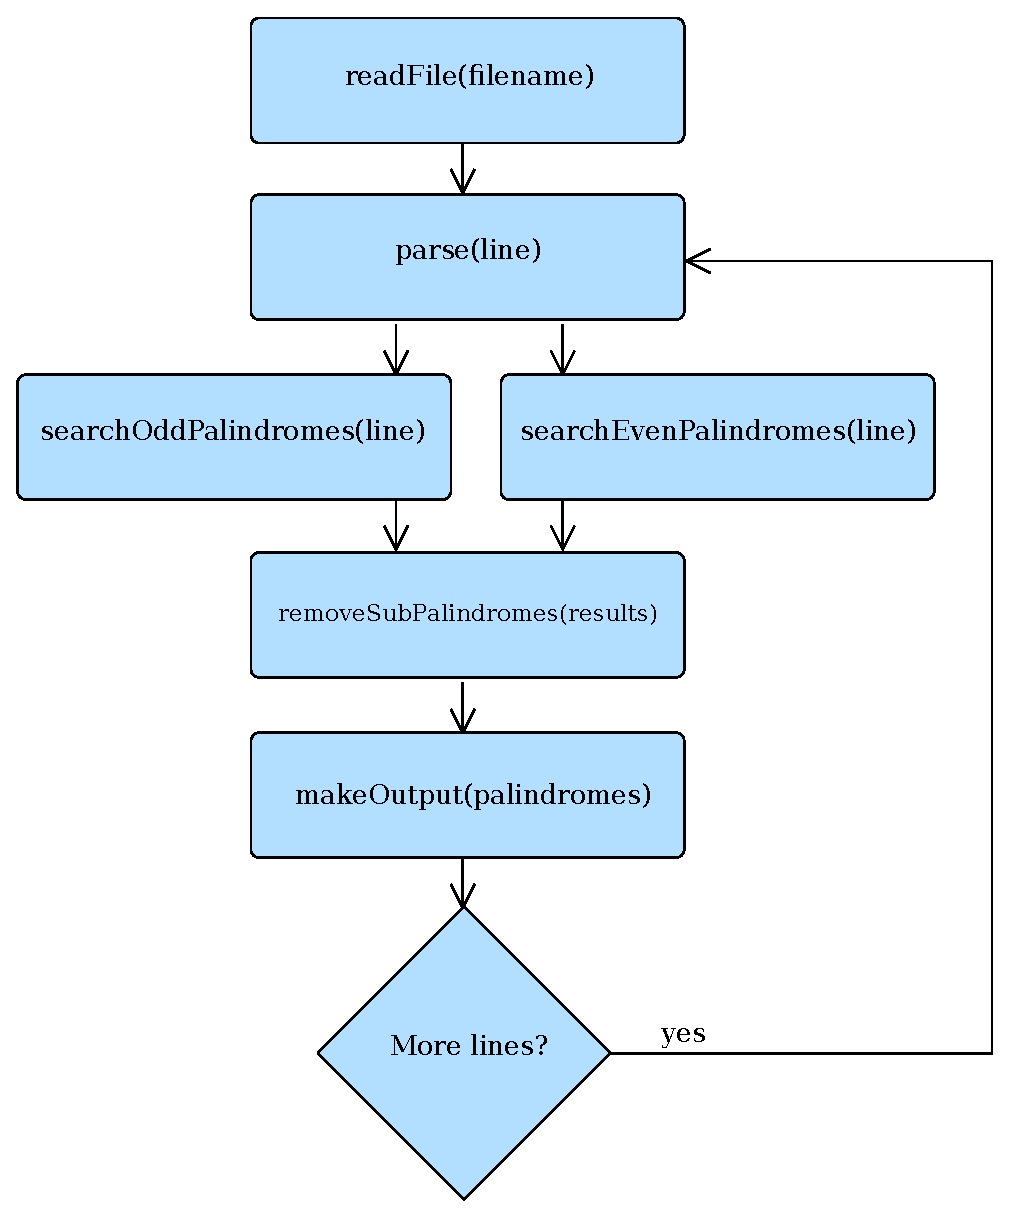
\includegraphics[width=0.9\textwidth]{FunctionalBlocks.eps}
  \vspace{-100pt}
\end{figure}

\newpage

\section{Pseudocode}
\vspace{-12pt}
\begin{verbatim}
readFile(Filename) ->
    Lines := open(Filename, 'r').read().split('\n'),
    Lines[:"QUIT"].

isPalindrome(String) ->
    case length(String) rem 2 of
        0 ->
        String[:length(String)/2] == reverse(String[length(String)/2:]);
        1 ->
        String[:length(String)/2] == reverse(String[(length(String)/2)+1:])
    end.

evenSearch(Line, Results) ->
    do stuff,
    ++Semaphore;

oddSearch(Line, Results) ->
    do stuff,
    ++Semaphore;

parseLine(Line) ->
    Semaphore = -1,
    Even = spawn(evenSearch(Line, Results, Semaphore)),
    Odd = spawn(oddSearch(Line, Results, Semaphore)),
    
    Semaphore.aquire();
    Results := filter(Results, (Palindrome) -> !isSubPalindrome(Palindrome)),
    Results.

main([Filename]) ->
    Lines := readFile(Filename),
    LineResults := [parseLine(Line) for Line in Lines],
    for LineResult in LineResults:
        print(''.join(LineResult))

\end{verbatim}

\end{document}
